% \title{ Сравнение подходов обучения на базе словаря и MAP к проблеме повышения разрешения на примере изображений автомобильных номеров }
\title{Повышение разрешения изображений автомобильных номеров}
\author{
  \begin{tabular}[4cm]{rl}
 Автор:                & Улитин А.~А., 461 гр. \\
 Научный руководитель: & доц.~Вахитов А.~Т.
 \end{tabular}
 }
\date{}

\begin{frame}{}
		\maketitle
\end{frame}

\section{Задача}
\begin{frame}{Задача Super-resolution}
  Задача Super resolution --- качественно повысить разрешения изображения.
  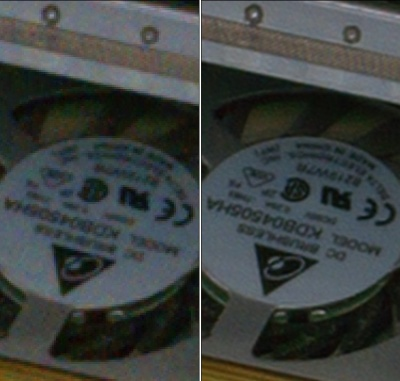
\includegraphics[height=\textheight]{content/An_example_of_super_resolution_with_still_RAW_photo.jpg}
\end{frame}

\begin{frame}{Почему это возможно}
  Для повышения разрешения используется дополнительная информация
  \begin{itemize}
    \item знание параметров съемки (размытие, движение камеры~и~т.п.)
    \item знание о типе снимаемого объекта (текст, лица, и т.п.)
    \item использование нескольких изображей, снятых с разных ракурсов
  \end{itemize}
  которая влияет на конечное изображение
\end{frame}

\begin{frame}{PSNR}

  $$ \mathrm{MSE}(\tilde{x},x) = \frac{1}{m\,n}\sum_{i=0}^{m-1}\sum_{j=0}^{n-1} [\tilde{x}(i,j) - x(i,j)]^2$$

  И обозначим величину обратную ей и выраженную на логарифмической шкале как $\mathrm{PSNR}(\tilde{x},x)$.
  $$ \mathrm{PSNR}(\tilde{x},x) &= 10 \cdot \log_{10} \left( \frac{\mathrm{MAX}_I^2}{\mathrm{MSE}(\tilde{x},x)} \right)
  $$

\end{frame}

\begin{frame}{Постановка задачи}
 $$y_r = D H_R W_R x + n_r,~ ~ ~ 1 \leq r \leq m$$
 где:
 \begin{itemize}
   \item $x$ оригинальное изображение
   \item $y_r$ наблюдение r
   \item $D$ матрица понижение разрешения
   \item $W$ матрица геометрического искажения
   \item $H_R$ матрица размытия наблюдения r
   \item $n_r$ шум наблюдения r
   \item $m$ количество наблюдений
 \end{itemize}
 Задача найти
 $$ \tilde{x} = \underset{\hat{x}}{\operatorname{argmax}}~  PSNR(\hat{x},x)$$
\end{frame}
\section{Подходы}
\begin{frame}{Сравниваемые подходы}
  \begin{itemize}
    \item Couple Dictionary Training for Image Super-resolution \\
        (Jianchao Yang,Zhaowen Wang, Zhe Lin,Scott Cohen, and Thomas Huang)
      \begin{itemize}
        \item использует пару тренированных словарей
        \item восстановление по одному изображению
      \end{itemize}
    \item Superresolution of License Plates in Real Traffic Videos \\
      (K. V. Suresh, G. Mahesh Kumar, and A. N. Rajagopalan)
      \begin{itemize}
        \item для восстановление использует последовательную оптимизацию с
          регуляризаторами
        \item использует несколько изображений
      \end{itemize}
  \end{itemize}
\end{frame}

\newcommand{\inimage}[2]{
  \begin{minipage}{#1}
    \vcenter{\includegraphics[width=\columnwidth]{#2}}
  \end{minipage}
}


% \section{Приведение изображений}
% \begin{frame}{Несколько изображение $\rightarrow$ одно изображение}
%   Для тестирования на однинаковых наборах данных из lr строились псевдо hr для
%   первого алгоритма методом:
%   $$ R = \frac{1}{n}\sum_{i=1}^nW^T \cdot S \cdot IMG_{lr i}$$
%   $S$ --- билинейная интерполяция \\
%   $W$ --- сдвиг
% 
%   \inimage{3cm}{content/imgs/append_imgs_big.jpg}
%   $\to$
%   \inimage{6cm}{content/imgs/combined_big.jpg}
% \end{frame}

\begin{frame}{Исходные изображения}
  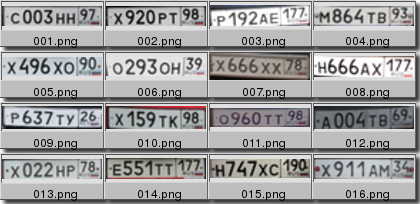
\includegraphics[width=\columnwidth]{content/out_sr1.png}
\end{frame}

\section{SR1}
\begin{frame}{Результаты подхода}
  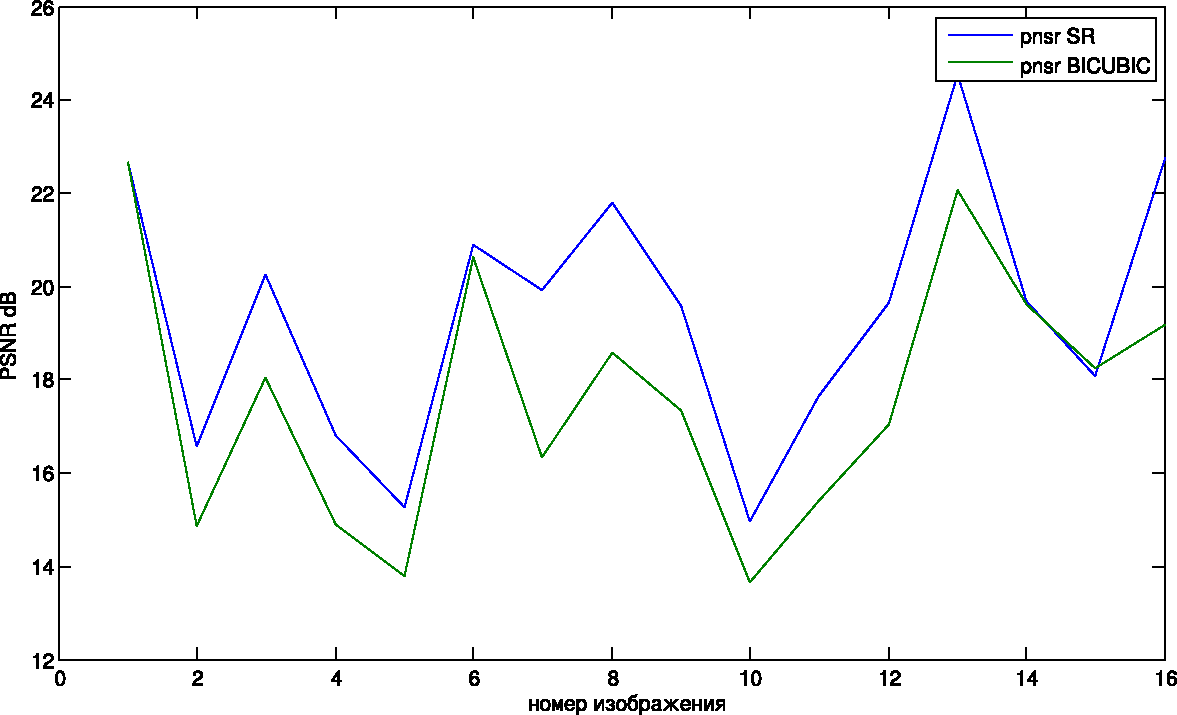
\includegraphics[width=\columnwidth]{content/pnsr_for_big_jpeg.pdf}
\end{frame}
\begin{frame}{Пример изображений SR1}
  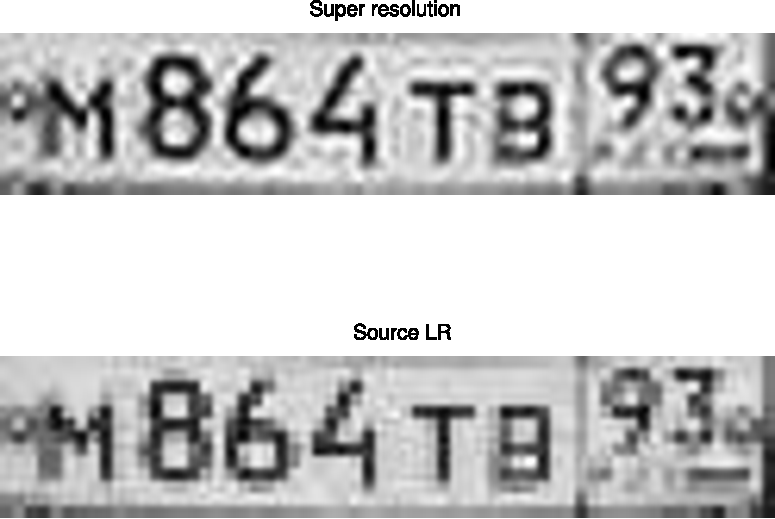
\includegraphics[width=\columnwidth]{content/compare_result_sr1.pdf}
\end{frame}

\section{RESULT 2}
\begin{frame}{Результаты подхода}
  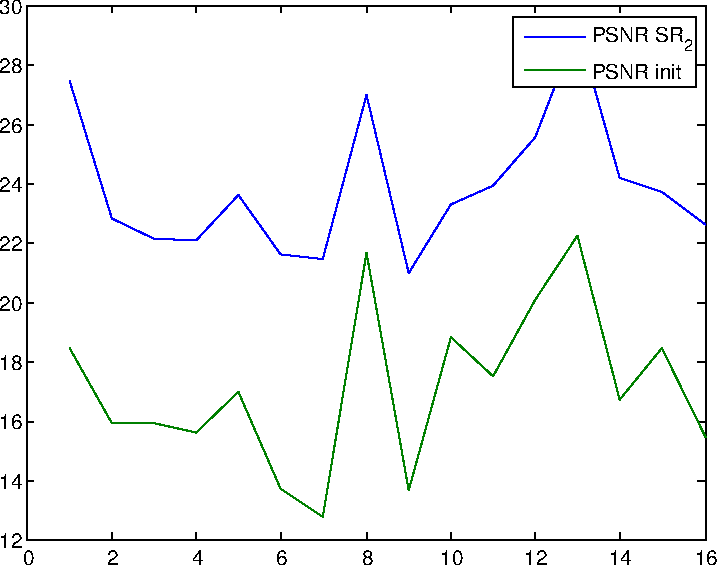
\includegraphics[width=\columnwidth]{content/compare_result_sr2.pdf}
\end{frame}
\begin{frame}{Пример изображений SR2}
  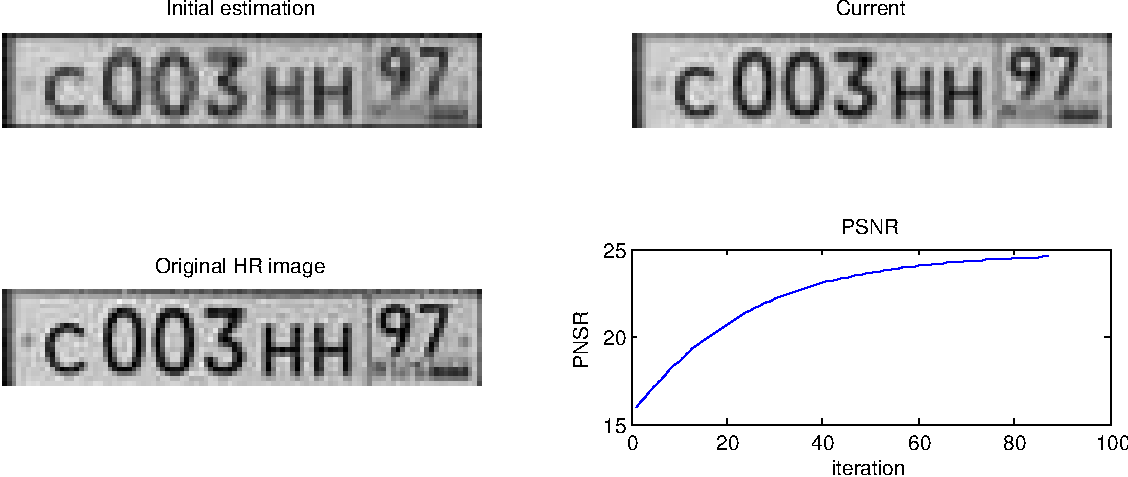
\includegraphics[width=\columnwidth]{content/sr2_result_img.pdf}
\end{frame}

\begin{frame}{Пример изображений SR2}
  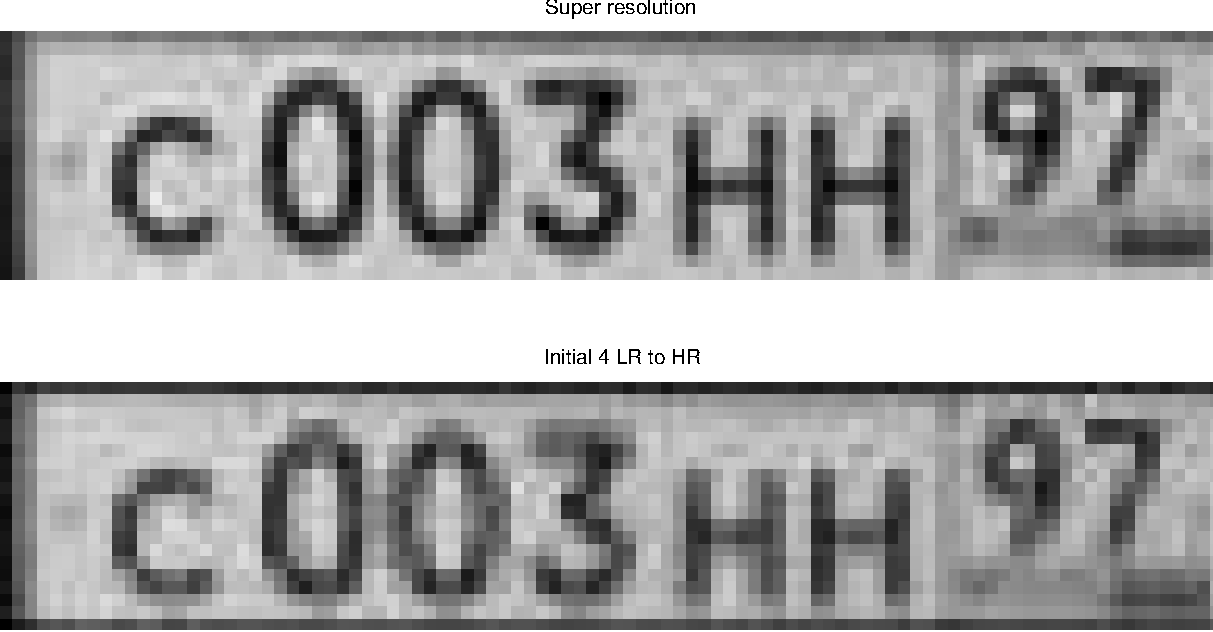
\includegraphics[width=\columnwidth]{content/sr2_two_images.pdf}
\end{frame}

\section{Итоги}

\begin{frame}{Итоги}
  \begin{itemize}
    \item были исследованы и реализованы два подхода к задаче SR
    \item эксперименты показывают, что оба алгоритма качественно повышают разрешения автомобильного
      номера.
  \end{itemize}
\end{frame}
